\documentclass[]{article}

\usepackage{lipsum}
\usepackage[margin=1in]{geometry}
\usepackage{graphicx} %Allows you to import images
\usepackage{float} %Allows for control of float positions
\begin{document}

\title{Seneka App\\
Universidad de los Andes\\
Airbus Fly Your Ideas}
\author{Garzón Miguel, Gómez Paula, Mendoza Santiago, Villegas Juan}
\maketitle


\Large{\textbf{1. Summary}\\}

Seneka is a platform with the ability of integrating the basic technology and engineering concepts in order to provide to the flight passengers the capacity of using their time in a pleasant way along the different airports that might be involved in their path during their business or leisure flights. Moreover, the platform brings support to the airport and airlines to allow them tracking, alerting and making contact with a passenger to notify about changes on their flight itinerary. Seneka also supports the interaction between passenger and the airport, a passenger can get notifications about the commercial offerings and the status of his order. Additionally, the passenger becomes an active member of the security team of the airport by informing to the local authorities about any emergency or misbehaviour from any other person using the app. The application has a sign-in interface for user that subsequently directs it to an airport selection interface where he or she will indicate where they want to be located and find optimal routes for their displacement. Likewise, the app has a search selection interface where the users can find stores, boarding gates and places of interest. Furthermore, an user profile interface can be found where it is possible to identify and modify their personal information and verify their flights.\\


\begin{figure}[H]
\centering
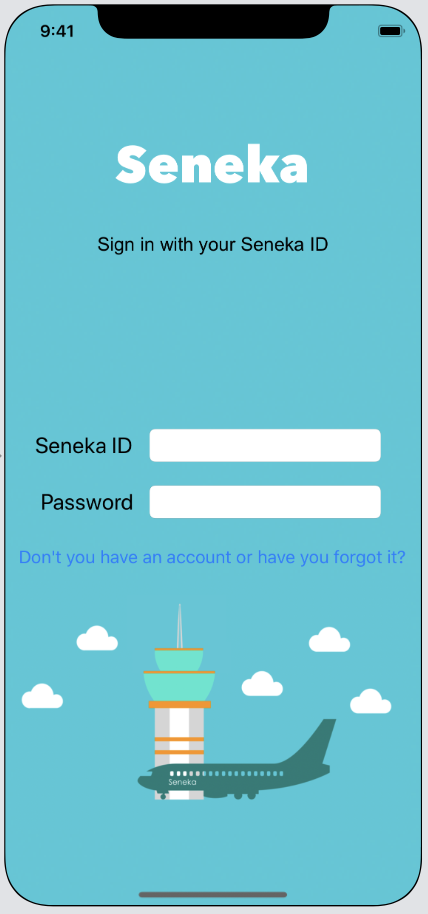
\includegraphics[height=4.0in]{Figura_1.jpg}
\end{figure}

\Large{\textbf{2. Objetives}\\}

\Large{\textbf{2.1 Main Objetive}\\}\\
[0.1cm]

Design a platform that can provide user support on his/her way through an airport by alerting, giving advice and a guidance through his/her corresponding routes within the airport, while giving secure communication channels between airports, airlines and passengers.\\
[0.7cm]

\Large{\textbf{2.2 Round 2 Specific Objetives}\\}
\begin{itemize}
	\item Design the business architecture which is consisted of the business canvas, the business ecosystem and the services brochure.
	\item Validate the acceptance of the idea throughout a market analysis based on surveys, existing companies and their success key factors.
	\item Create a functional sign-in interface based on the results of the design analysis (Colors and requirements). 
	\item Develop a broaden knowledge of the technical specifications for the mapping and location of the user.
	\item Develop a previous map interface to visualize the application on a phone.\\
[0.7cm]
\end{itemize}

\Large{\textbf{2.3 Round 3 Specific Objetives}\\}
\begin{itemize}
	\item Create a functional map interface to guide a passenger to a desired place and find commercial offers through a foreing airport.
	\item Implement a security bottom thar make the passenger connect inmediately with police or nearly security guard on the airport.
	\item Implement an "alert flight status" that gives a warning message to the passenger regarding flight status, delays and board gates updates. 
	\item Based in service brochure, we will develope an app which could be used in a cell phone with iOS system.\\
[0.7cm]
\end{itemize}

\Large{\textbf{3. Description}\\}\\


\Large{\textbf{4. Summary}\\}\\


\Large{\textbf{5. Outcomes}\\}\\


\Large{\textbf{5.1 Achievements}\\}

The aeroespace industry will get stronger as the number of passengers could feel confortable with the security and good service. But the aeroespacial industry also includes ground service and people working in it, that is one of the aspects that might have been forgotten or neglected. With Seneka platform and its service Seneka App, passengers, airports and airlines could be beneficiaries of the system of tracking paths within the airport, that's because people could be more in touch with all the services offered inside of it.\\

Likewise, sales will increase with the arrival of more and new travelers that are more likely to go through this airport with the revolutionary Seneka's way to buy at the airports around the world. The system is easy, the passenger select his/her products and pays in the platform. Then enters his route and the app locates the nearest cupboard in which she/he could get his purchase without going trough the airport. The cupboard are the new spaces that we identify as a pick up station, in which the seller leaves the purchase with a security code that buyer already has. Putting this code, the cupboard autmatically selects the order and deliver it to the buyer in a few seconds.\\

At the same time, the congestion on hours of simultaneous boarding flights will be better as the number of travelers using Seneka App increases, because they will get an efficiet path to get into the correct gate. The waiting rooms will get full only at the right times because passengers will spent their time in entertaimen places without fear of losing their fligths.




\end{document}
